As the title suggest, this chapter describes the design process and the resulting experimental system setup. Section \ref{sec:setup} describes the general overview of the experimental setup: subsystems that builds the whole experimental system, the ``job description'' of each subsystems, and how each subsytems relate to each other to run the whole experimental system. Sections \ref{sec:trans}, and \ref{sec:measure} describes in detail the components, how each components work, and how those components relate to each other to build translational, rotational, force measuring, respectively. The last section (Sec. \ref{sec:specimenmodel}) describes the specimen that was used in this thesis, including design consideration, production process and it's mechanical properties.\par
\section{Experimental Setup in General}
\label{sec:setup}
The experiment was conducted in towing tank facility in Aerogasdynamics Laboratory in Aerospace Engineering programme, Faculty of Mechanical and Aerospace Engineering, Bandung Institute of Technology. The towing tank is glass-walled and 200 $\times$ 60 $\times$ 60 cm in length, width, and height, respectively. The towing tank was filled with typical water (density $\rho$ = 1000 kg/m$^{3}$ and kinematic viscosity $\nu$ = 1 $\times$ 10$^{-6}$ m/s$^{2}$) up to 43 cm in height. A carbon fiber carriage was attached to two shafts with four linear bearings above towing tank to carry a specimen, a servo for rotational motion, and a load cell for force measurement. The carriage was connected via belt-and-pulley mechanism to a stepper motor for translational motion.\par
The experimental system can be divided into three major subsystems: traversing system for moving the specimen along translational (i.e forward and backward) plane, force measurement system for measuring the instantaneous force acting on the specimen. Figure \ref{fig:schemeexpforce} describes the relationship between each subsystems to build the experimental setup for force measuring purpose. These subsytems will be explained in detail in the following sections.
\begin{figure}[H]
    \centering
    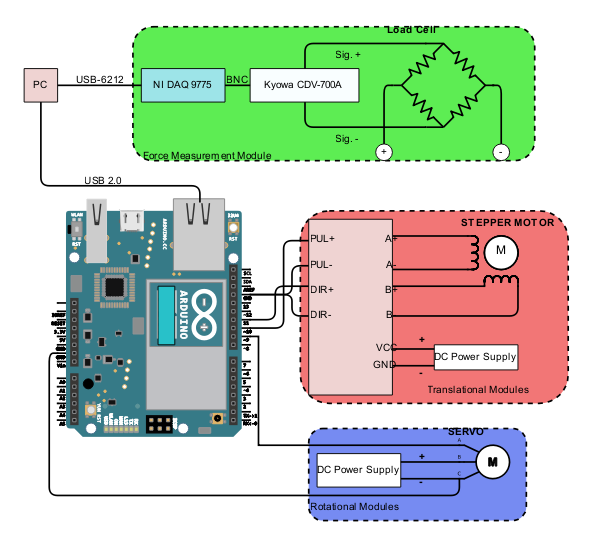
\includegraphics[scale=0.75]{schemeexpforce.png}
    \caption{Subsystem schematic for force measurement experimental runs.}
    \label{fig:schemeexpforce}
\end{figure}
It is also worth noting that it is desirable to have an automated experimental system, which means that all system must be connected to a personal computer and controlled by a software. In this case, the hardware controller used was an Arduino Uno R3 board. Arduino is a microcontroller board based on ATmega328, an AVR 8-bit processor, esentially a mini computer suitable for repeating tasks. Arduino Uno has 14 digital I/O pins, 6 of which can be used as PWM outputs, and 6 analog input pins. The softwares are Arduino package for traversing system and MATLAB R2015a for data and image acquisition and also optimisation algorithm. In traversing system, Arduino Uno R3 board was used to connect stepper motor and servo motor to a personal computer and a code was built to control both motors. A code based on Arduino language (which in turn is based on C++) was made as an interface between user, computer, and hardwares related to traversing purpose and a code in MATLAB was built as an interface for data acquisition and optimisation needs. Both of those softwares communicate through serial communication native to Arduino and MATLAB. The towing tank facility can be seen in figures \ref{fig:setupirl} and \ref{fig:setupdatairl}.
\begin{figure}[H]
    \centering
    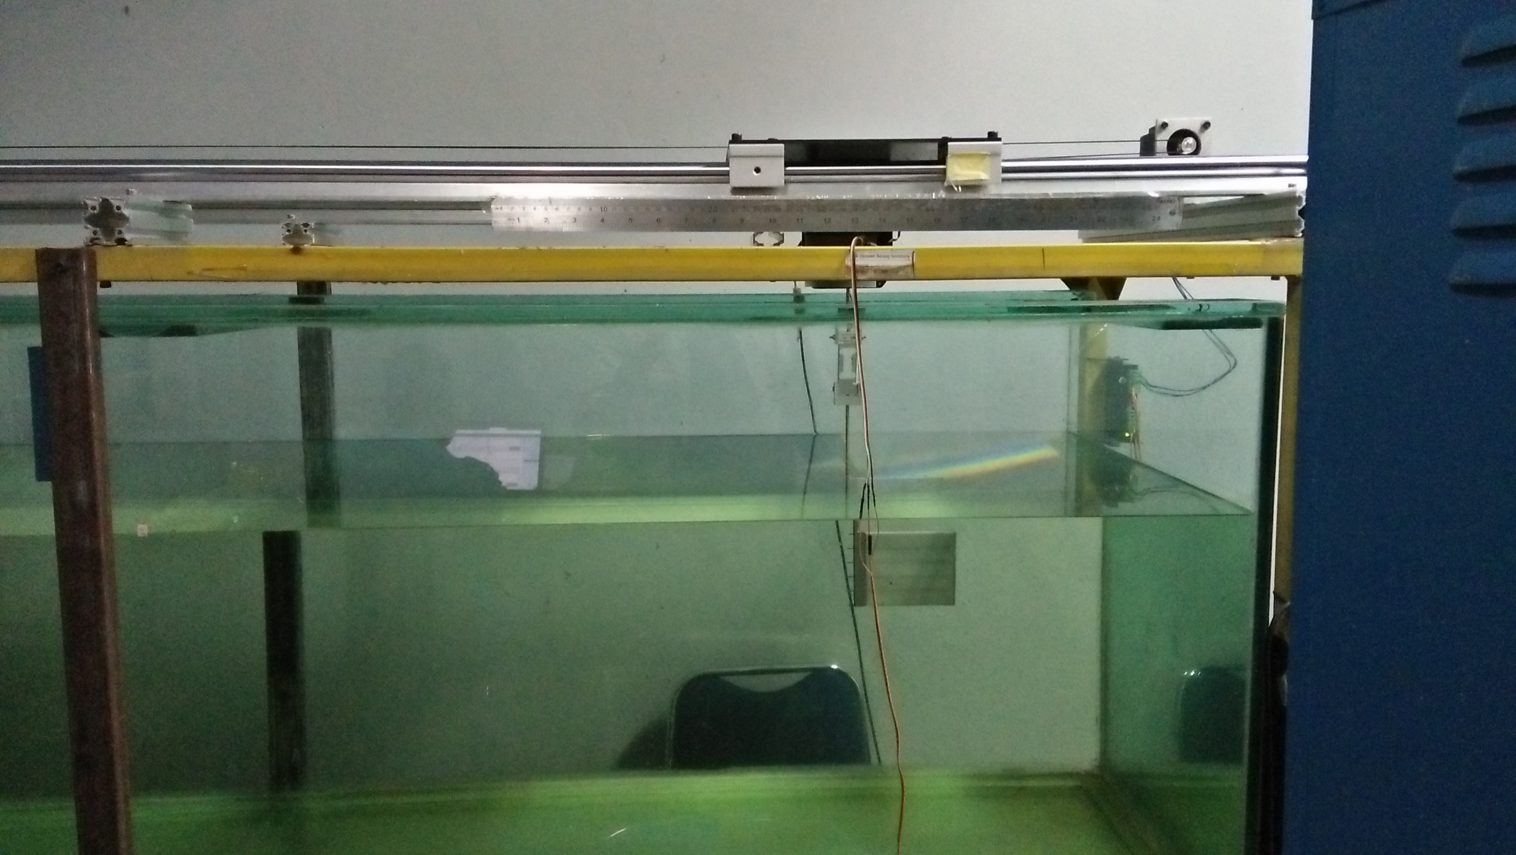
\includegraphics[scale=0.6]{setupirl.png}
    \caption{Towing tank experimental facility.}
    \label{fig:setupirl}
\end{figure}
\begin{figure}[H]
    \centering
    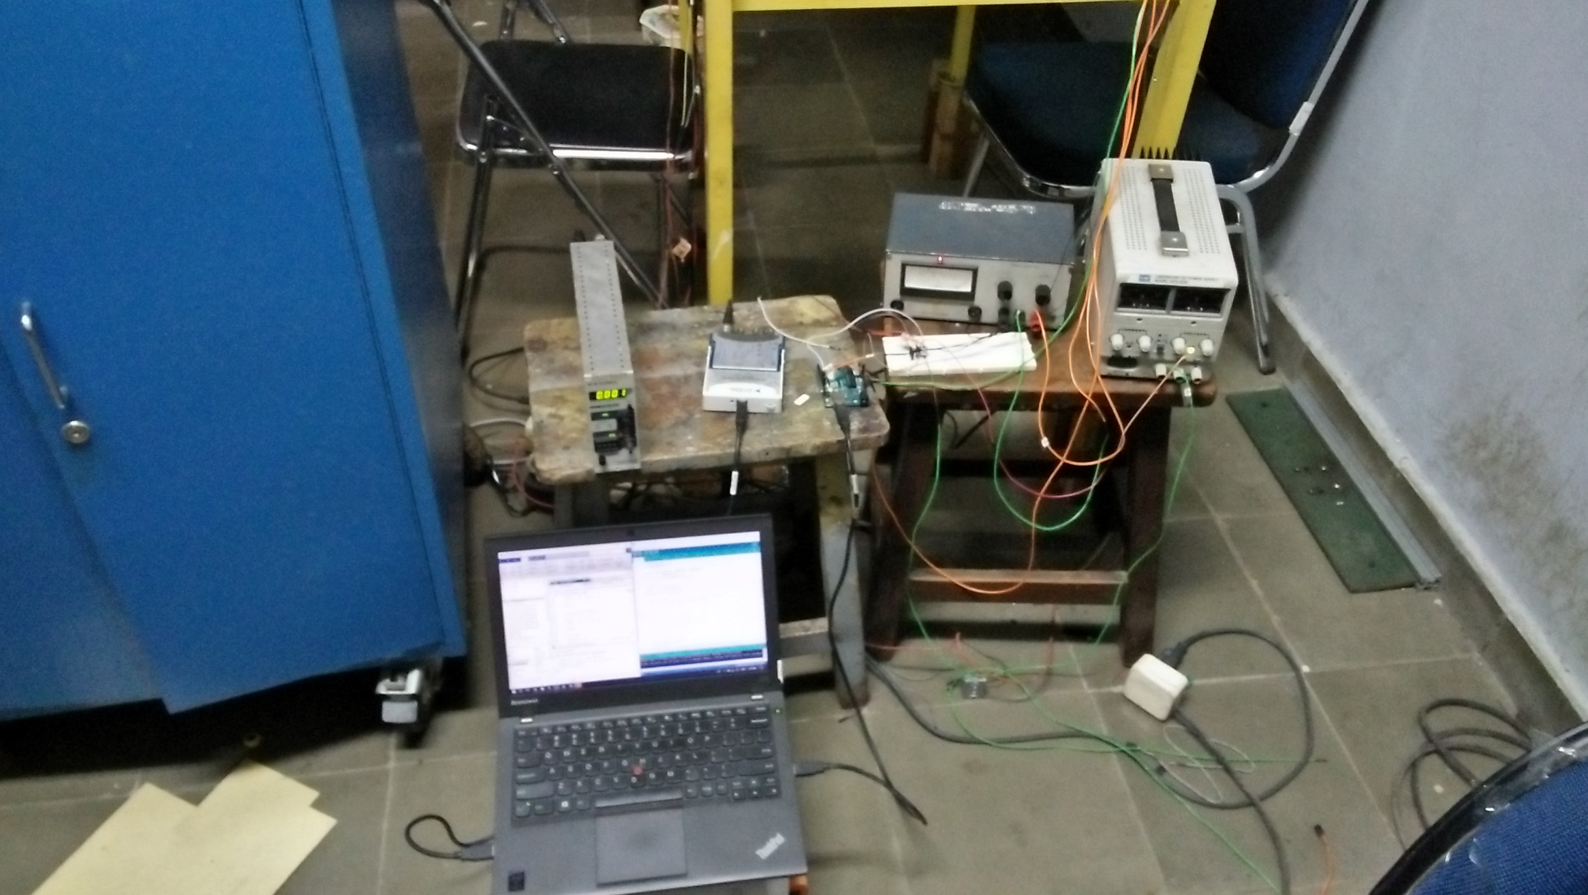
\includegraphics[scale=0.6]{setupdatairl.png}
    \caption{Towing tank experimental control panel.}
    \label{fig:setupdatairl}
\end{figure}
\section{Traversing System}
\label{sec:trans}
Traversing system dictates how does the specimen moves forward, backward, and rotates during the duration of experiment. This system is further divided into two smaller systems: translational system, described in subsection \ref{sec:forback}, which deals with how does a specimen moves forward and backward, and rotational system, described in subsection \ref{sec:rotate} which deals with how does a specimen moves rotationally.
\subsection{Translational System}
\label{sec:forback}
Translational system is indicated with red background on figures \ref{fig:schemeexpforce} and \ref{fig:schemeexpimage}. The system consists of one stepper motor, one stepper motor driver, and one DC power supply. The system was designed to move the carbon fiber carriage backward and forward on a straight line. To do that, the carbon fiber carriage was mounted on four 20 mm linear bearings which in turn rest on two 20 mm circular shafts. The carbon fiber carriage was also connected to two pulleys on both ends of the water tank via a 2 mm pitch rubber belt. On one end, a timing pulley with matching pitch was mounted on stepper motor shaft and on the other end a pitchless idler pulley was mounted on a custom aluminium frame. The correlation between motor rotational speed in rps (rotation per second) denoted by $\omega$ and resolution of microstep (i.e how many pulses are generated for one motor shaft revolution) denoted by $n$ is:
\begin{equation}
    \omega = \frac{f}{n}
    \label{eq:pprtorotspeed}
\end{equation}
where $f$ is the input pulse frequency. For this experiment, the resolution of microstep was set at 1600 pulse/rev and the driver is rated at maximum 200 kHz pulse frequency. Therefore, the translational speed of the carriage can be written as:
\begin{equation}
    v = \pi\omega d
    \label{eq:omega2vel}
\end{equation}
where $d$ is the diameter of the motor shaft, $d$ = 6.35 mm. It should be noted that controlling the velocity and distance traveled by the carriage, manually adjusting the pulse input or microstep resolution is not required. A more convenient method is to use a native Arduino library to control direction, distance, and velocity \texttt{\textcolor{blue}{<AccelStepper.h>}}.\par
A Leadshine NEMA23 2-phase stepper motor was connected to Leadshine DM542 stepper motor driver pins following the available manual written in the stepper motor. The stepper motor was powered using a DC power supply connected to V+ and GND pin for positive voltage and negative voltage, respectively. The power supply was able to supply 0 - 50 V DC and the stepper motor driver itself requires minimum 20 V DC to operate. The rest of the pins was connected to digital input pins on an Arduino R3 Uno board. PUL+ pin which generates the pulse or step needed to rotate the motor shaft was connected to digital pin number 10 on Arduino R3 Uno board, DIR+ pin which governs the direction of motor shaft rotation (i.e clockwise or counter-clockwise) was connected to digital pin number 11, PUL- and DIR- were connected to GND pin.\par
\subsection{Rotational System}
\label{sec:rotate}
To mimic oscillating motion of a fin, rotational system was designed to fulfill said purpose. This system can rotate fin panel by rotating the load cell which was placed above the fin panel supported by a circular bar. This motion was actuated using Futaba S3003 servo placed inside a box along with two roller bearings attached inside the box to keep the circular bar supporting the fin straight. Two connectors held the bar between servo motor and the circular bar which was attached to the fin panel. The servo was powered by a laboratory power supply providing 5V. The positive terminal in the power supply was connected to the positive cable of the servo, the negative terminal was connected to the grounding terminal of the servo and was branched with a breadboard to be connected to the power ground in the Arduino board. The signal pin in the servo was connected to digital pin number 9 in the Arduino. Depicted in figure \ref{fig:rotvisual}, servo could change angle $\theta$ from $0^{0} - 180^{0}$ measured from a vertical line perpendicular to the translation direction by responding to a pulse length modulation with short duration between 1 - 2 ms. The motion of the servo was controlled using \texttt{\textcolor{blue}{<Servo.h>}} library native to Arduino.
\begin{figure}[H]
    \centering
    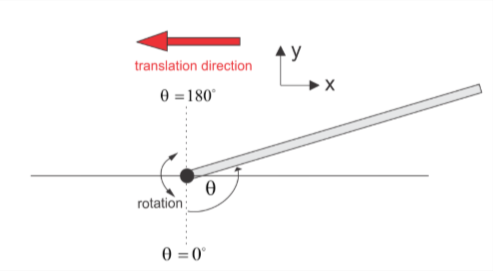
\includegraphics[scale=0.75]{rotvisual.png}
    \caption{Fin panel motion depiction.}
    \label{fig:rotvisual}
\end{figure}
\section{Force Measurement System}
\label{sec:measure}
An aluminium 300g single point load cell PW4MC3 (HBM) combined with Kyowa CDV-700A signal conditioner acted as two main component for force measuring. The load cell was used to measure the force acting on fin panel during it's motion and the signal conditioner acted as a signal amplifier and lowpass filter. Along with these two components, National Instruments DAQ board was used for data acquisition and this board was connected to a personal computer using USB-9215A which also acted as analog-to-digital converter which transmit sgnals from force measurement (an analog signal) to a personal computer (reads digital signal). The load cell has accuracy class C3 with OIML R60 test report and minimum sensitivity at 3 mN and the signal conditioner was operated in 2V bridge excitation voltage, RANGE in the value of 500 and 10 Hz cut-off frequency for analog lowpass filter.\par
As stated in section \ref{sec:rotate}, the load cell also rotates with fin panel, which means that the force data read by the load cell is force acting parallel to the chord line of the fin panel (denoted by $F_{load}$) in figure \ref{fig:freebodydiag}.
\begin{figure}[H]
    \centering
    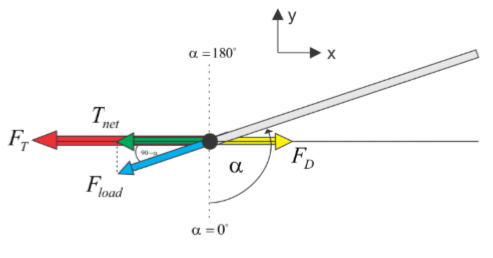
\includegraphics[scale=0.75]{freebodydiag.png}
    \caption{Free body diagram of forces acting on fin panel on xy-plane.}
    \label{fig:freebodydiag}
\end{figure}
Figure \ref{fig:freebodydiag} visualise forces acting along the translation direction experienced by the fin panel. The oscillating motion of the panel produce thrust force $F_{T}$ while drag force $F_{D}$ is the consequence of the panel translational motion. $F_{load}$ can be transformed into net thrust force $T_{net}$ by taking the x-direction component of $F_{load}$:
\begin{equation}
    T_{net} = F_{load} \cos \left(\alpha - 90\right) = F_{load} \sin\alpha
    \label{eq:load2net}
\end{equation}
The raw data obtained from load cell measurement was processed further to eliminate noise inherent to electrical systems. This was accomplished by imposing a digital lowpass filter to the raw data. The filter design was based on Butterworth n-th order filter with $f$ cutoff frequency, in this case, the filter order was chosen to be 4 and the cutoff frequency was specified at 2 Hz. The cutoff frequency value was determined from power spectrum density graph and the filter order was obtained based on previous thesis by \citet{hiroki}. The smoothing process was done using moving average method where the first element of each data was determined by taking the average of $n$ points forward. In the experiment, the points used to smooth the n-th data was determined at 100 points. This value was obtained through trial-and-error process.
\section{Variable-Stiffness Fin Model}
\label{sec:specimenmodel}
The fin model (Fig. \ref{fig:finpanel}) with varying stiffness was made using a 80 $\times$ 100 mm silicone rubber with six spring steel wires embedded within the silicon rubber during the production process. These spring steel wires acted as stiffeners and the stiffness of the whole specimen was varied by changing the length of the wire. This fin panel was glued to an aluminium board with matching thickness to prevent the fin panel from shearing, making sure that the flapping motion was strictly limited to flapping only. This board has six threaded holes on one of its surface that was used to prevent the wires from moving during flapping motion. The board was attached to the load cell with a 4 mm diametre circular bar and some part of the bar was lathed to fit the thickness of the fin (thickness = 3 mm) and to reduce the drag induced by the presence of the bar. The board and the bar was again glued to prevent the fin from slipping as slipping motion results in different amplitude output given a particular input.
\begin{figure}[H]
    \centering
    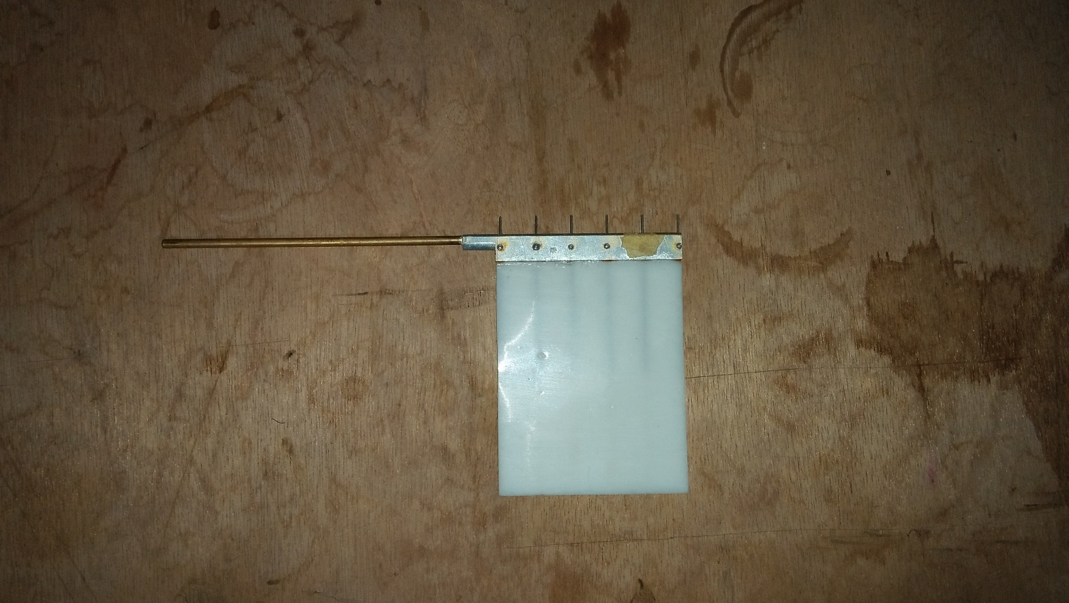
\includegraphics[scale=0.75]{specimen.png}
    \caption{The fin panel end product.}
    \label{fig:finpanel}
\end{figure}

The fin panel was made by pouring a 1:25 volumetric mixture of silicone rubber and catalyst ($E$ = 0.08 GPa) that had been vaccuumed in a pressurised vessel to a die made from acrylic boad matching the fin panel dimension. Within the die, six spring steel wires ($E$ = 207 GPa) was attached horizontally at it's ends that acts as the stiffener chord-wise and two wires was attached vertically at the leading and trailing edge to ensure stiffness along the thickness, thus ensuring that the panel does not twists as it flaps. The mixture inside the die was then vaccuumed again inside a pressurised vessel to ensure that there are no voids trapped inside the fin panel which may results in different material properties along the panel.\par
Changing the stiffness of the fin panel was simple: changing the spring wires length also changes the distribution of the material stiffness chord-wise, where the change of the material distribution also change the stiffness distribution which also leads to effective stiffness change of the whole panel. The wires was fastened using 1.27 mm set screws attached to six threaded holes in the aluminium board to keep the wires in place during motion. Changing the length was simply done by first loosening these set screws and pulling the wires using a pliers from the leading edge until the desired length and then refastened the set screws. To ensure the wires is already at the desired length, another wire was put inside the silicone from the trailing edge. This wire has a marking that indicates the previously desired wire length and if the wires barely touch each other, then the wire has reached the desired length.